%!TEX root = Memoria_TFM.tex
\section{Anti-spoofing and biometrics systems}
At the same time as technology advance, capture systems and processing algorithms have proceed too. This open an immense options quantity and one of them is the capability of developing more sophisticated identification systems, giving way to biometrics systems.\\

\subsection{Historical introduction}
There were in the 1870s when the necessity of identifying people getting physical characteristics appeared. Alphonse Bertillon had the desire of identifing jail prisoners, in order to do that, the skull diameter, arm and foot length were utilized for that purpose in USA until the 1920s \cite{Intro_biometrics}.\\

 There were in the 1880s when fingerprint and facial identification were proposed. But with the appearance of digital signals processing systems in 1960, the voice and the fingerprint biometric systems were started to be investigated and researches started to think to use this system to identification in access control security \cite{Intro_biometrics}.\\
 
Ten years later, the geometry of the hand was started to be a field of interest for automated technologies of identification. The retina and signature verification appeared in the 80s and after a short time the face systems \cite{Intro_biometrics}.\\

 The last biometrics systems appeared in the 1990s with the iris recognition \cite{Intro_biometrics}.\\

\subsection{BLAAAAAA}
Some biometrics systems have been mentioned above. Each one uses a specific part of the human body to identify or verify an identity. But there are more biometrics than the described above as the veins or the ear.\\

As the same time as biometrics authentication systems appeared, the attacks to trick systems emerge and they are called \textit{spoofing attacks}. For example making plaster molds for geometric hand biometrics or fingerprints would be an attack as the presented in figure \ref{fig:Spoof_fingerprint} (image has been obtained from \cite{fingerprint_image}).\\


\begin{figure}[htb]
\centering
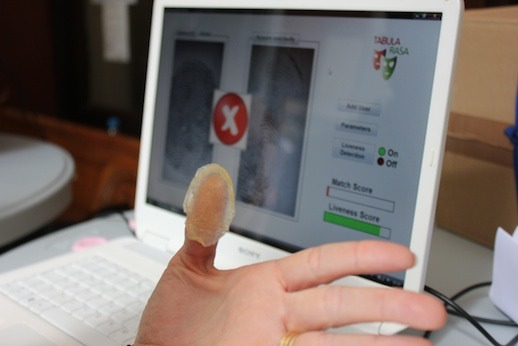
\includegraphics[width=0.5\textwidth]{images_miscelaneus/spoofing_fingerprint.jpg}
\caption{Spoofing fingerprint. Image obtained from \cite{fingerprint_image}} \label{fig:Spoof_fingerprint}
\end{figure}

Spoofing is referenced to create a new and genuine identity or impersonate a system. The attack would depend on the biometry and the capturing system \cite{Spoofing_survey}.\\

In order to get the tricks and do not allow spoofing attacks, \textit{anti-spoofing} tries to minimize the attacks or prevent them.\\

There are two ways of evaluating anti-spoofing scenarios \cite{Spoofing_survey}:
\begin{description}[noitemsep,topsep=8pt,parsep=0pt,partopsep=20pt]
\item \textbf{Algorithm-based or technology evaluation:} to evaluate algorithms or liveness detection.
\item \textbf{System-based or scenario evaluation:} to evaluate the entire acquisition systems.
\end{description}

When an identification or biometric system is used two general task could perform:
\begin{description}[noitemsep,topsep=8pt,parsep=0pt,partopsep=20pt]
\item \textbf{Recognition:} when the system, from the input, has to decide the identity of the user (name, ID,...)
\item \textbf{Verification:} when the system is given a determined identity and has to decide if it is the genuine or is a person trying to supplant the identity.
\end{description}

In this project it is going to be developed the algorithm to detect anti-spoofing attacks when the face is using as biometrics. Given an image, the system has to decide if it is an attack or a genuine user. It would be a verification task.\\

\subsection{Face anti-spoofing}
Face is a very used biometric system and also it is one of the most attacked biometrics because of the fact that the capturing system for face biometrics could be as simple as a RGB camera, so a printed photo or an image in a smartphone could be easy to acquire as spoofing attacks. Otherwise, a spoofing attack for an vein biometrics is more sophisticated than a printed photo.\\

The principal or main used acquire system are RGB cameras although other cameras as infra-red  or depth camera are used too. Using different types of camera could help to detect anti-spoofing attacks. The main used attacks for this biometric is a printed image or a mask and displaying a photo or video in a smartphone or tablet and its cost is low \cite{distorsion}.\\

Two big advantages of this biometric are the non-intrusive method and the positive acceptance of this biometric in society. On the other hand, compare frontal face with faces with a determined angle is not as well managed as compared frontal with frontal faces \cite{survey2}.\\

\subsection{Related Works}
There are a lot of research work in face anti-spoofing and different method has been tested in researches.\\

Deep learning has been used to detect spoofing attacks. Convolutional neural networks are used to extract features and be allowed to differenciate between genuine and fake users. In \cite{LSTM-CNN} A LSTM-CNN has been developed, where the input in stead of being images are video and the network learn temporal features. In \cite{Verification} the purpose is the verification task, where the input are two images and the convolutional neural network is a Siamese. Another Anti-spoofing research with deep learning is the developed in \cite{yangLL14} where a simple Convolutional neural network has been developed to difference between genuine and no-real users.\\

Not only deep learning has been used with this purpose. The extraction of texture-based features (LBP, HOG, DoG,..) for face anti-spoofing have been researched \cite{distorsion}. In \cite{LBP_FaceAnti} authors study Local Binary Patterns (LBP) and variants of this method for face anti-spoofing.\\

Also the motion has been used. The lip movement, the head rotation or the blink eyes \cite{distorsion}. In \cite{Blink_antispoofing} is the blink movement of the eyes what authors use for face anti-spoofing.\\
